%% PNAStwoS.tex
%% Sample file to use for PNAS articles prepared in LaTeX
%% For two column PNAS articles
%% Version: Apr 15, 2008 
 

%% BASIC CLASS FILE
\documentclass{pnastwo}

%% ADDITIONAL OPTIONAL STYLE FILES
\usepackage{graphicx}
\usepackage{pnastwoF}
\usepackage{amssymb,amsfonts,amsmath}
\usepackage{bm}
%\usepackage[comma,sort&compress]{natbib}
\usepackage{cite}
\renewcommand\citeleft{(} \renewcommand\citeright{)}

%% OPTIONAL MACRO DEFINITIONS
\def\s{\sigma}
\newcommand{\erf}{\operatorname{erf}}


%%%%%%%%%%%%
%% For PNAS Only:
\url{www.pnas.org/cgi/doi/10.1073/pnas.0709640104}
\copyrightyear{2008}
\issuedate{Issue Date}
\volume{Volume}
\issuenumber{Issue Number}
%\setcounter{page}{2687} %Set page number here if desired
%%%%%%%%%%%%

\begin{document}

\title{Model-based transcription factor target
  identification without perturbations}

\author{Antti Honkela\affil{1}{Department of Information and Computer
    Science, Helsinki University of Technology, Finland}, Neil
  Lawrence\affil{2}{School of Computer Science, University of
    Manchester, UK}, Charles Girardot\affil{3}{Genome Biology unit,
    European Molecular Biology Laboratory, Heidelberg, Germany} Eileen
  E. Furlong\affil{3}{} \and Magnus Rattray\affil{2}{}}

\contributor{Submitted to Proceedings of the National Academy of Sciences
of the United States of America}

\maketitle

\begin{article}
\begin{abstract}

\end{abstract}

\keywords{transcriptional regulation | gene expression | systems biology | Gaussian process inference}

\abbreviations{TF transcription factor; ChIP Chromatin Imunnoprecipitation;}

\dropcap{T}ranscription factors are key nodes in the gene regulatory
networks that determine the function and fate of
cells. An important first step in uncovering a gene regulatory network
is the identification of target genes regulated by a specific
transcription factor (TF). A
common approach to this problem is to experimentally locate physical binding
of TF proteins to DNA sequence {\em in vivo} using a genome-wide
chromatin imunnoprecipitation (ChIP) experiment. However, in such an
experiment it is likely that many observed binding events do not
correspond to actual gene regulation and bound enhancers may be
distant from the promoter region of the gene that they control. Therefore, the task of identifying transcriptional
targets usually requires the integration of ChIP binding predictions
with evidence from expression data to help associate binding events
with target gene regulation. If there is access to expression data from a mutant in which the TF has
been knocked out or over-expressed, then differential expression of genes between wild-type
and mutant is indicative of a potential regulatory
interaction. The relationship of spatial expression for the
TF and putative target can also provide support for a hypothesised
regulatory link, where available. 

A problem with the above approach is that the creation of mutant
strains is challenging or impossible for many TFs of interest. Even
when viable mutants are available then they may provide very limited information due to the
confounding of signal from indirect regulatory feedback. For these reasons it
is useful to seek other sources of evidence to complement ChIP binding
predictions. In this contribution we demonstrate how a dynamical model of wild-type transcriptional
regulation can be used for genome-wide scoring of putative target genes. All that is required to apply
our method is wild-type time series data collected over a period
where TF activity is changing. Our approach allows for complementary
evidence from expression data to be integrated with ChIP binding data
for a specific TF without carrying out TF perturbations. 

To score putative targets we use the data likelihood under a simple
cascaded differential equation model of transcriptional regulation. The regulation model
we apply is ``open'' in the sense that we do not explicitly model regulation of the TF
itself. To deal with this technical issue we use a recently developed
non-parametric probabilistic inference methodology to
effectively deal with open differential equation
systems~\cite{Gao2008}. We model the TF concentration as a function
drawn from a Gaussian process prior distribution~\cite{Rasmussen2006}. This functional prior can either be placed
on the TF mRNA, for TFs primarily under transcritptional regulation,
or the TF protein, for TFs activated post-translationally. In the
application considered here the TFs are transcriptionally regulated
and we take the former approach. We use Bayesian marginalisation (also
known as Bayesian model averaging) to
integrate out this functional degree of freedom. This greatly reduces the
number of parameters required to model the data, making a
likelihood-based approach feasible even for relatively small
datasets. 

There are many existing approaches to inferring gene regulatory networks from
time-series expression data, including dynamic Bayesian networks,
information theoretic approaches and differential equation approaches
(reviewed in \cite{Bansal2007a}). These methods typically require many
more data from a greater diversity of experimental conditions than are
available from the short unperturbed wild-type time series that we
consider. However, our goal is more limited in scope since
we are primarily interested in providing additional support for hypothesised
targets of a specific TF. Again, most approaches to this problem are
designed for data containing large numbers of diverse conditions, as
exemplified by DREAM 2 target identification
challenge~\cite{Stolovitzky2007} (challenge 1). Others
have addressed this target identification problem using time-series
data with a regulation model~\cite{Barenco2006a,Gatta2008}. However,
these approaches either require a known target set for training~\cite{Barenco2006a} or
they require measured TF protein data~\cite{Gatta2008}. As well as
these differences in the assumed prior knowledge and data available,
it is also difficult to validate other approaches on the same data used in these
studies as they only carried out validation of positive targets
that they identified, rather than using unbiased genome-wide
experimental validation. 

We validate our proposed method by comparing the model-based target
ranking with published ChIP-chip data for two TFs controlling early
mesoderm development in Drosophila. Our method is shown to be comparable
to, or outperform, the use of knockout mutant data which are available
for these TFs. We demonstrate that a model-based approach is significantly
better than a simpler approach using correlation with TF
expression. We further show how integrating complementary wild-type spatial
{\em in situ} expression data can greatly improve target ranking accuracy. 

\section{Gaussian process inference for a linear activation model}

A Gaussian process is a probability distribution over
functions $f$ which take the value $f(t)$ at some particular time
$t$. Analogous to the Gaussian distribution, which is fully characterised by a mean and variance, the Gaussian process is
characterised by a mean function $\mathrm{E}[f(t)]$ and a covariance
function $k(t,t')=\mathrm{E}[f(t)f(t')]-\mathrm{E}[f(t)]\mathrm{E}[f(t')]$
where the expectation is over function evaluations at times $t$ and
$t'$. 

For the prior distribution of TF mRNA concentration profile $f$ we use a zero-mean squared exponential covariance
$k(t,t')=a\exp(-(t-t')^2/l)$. Samples from a Gaussian process with this choice
of covariance are smooth, infinitely differentiable, stationary functions. Although single-cell mRNA counts may be low
and vary in a highly stochastic manner, here we consider microarray data which
corresponds to a population average and is therefore more
appropriately modelled using a smooth process. The parameters $a$ and
$l$ describe the typical amplitide and time-scale of samples from
the prior. 

To simplify the inference we model translation and transcriptional
activation as simple linear processes using ordinary differential
equations,
\begin{align}
  \frac{\mathrm{d}p(t)}{\mathrm{d}t} & = f(t) - \delta
  p(t) \ , \label{eq:translation_ode} \\
  \frac{\mathrm{d}m(t)}{\mathrm{d}t} & = B+Sp(t)-Dm(t) \ , \label{eq:transcription_ode}
\end{align}
where $p(t)$ is the TF protein and $m(t)$ is the target mRNA
concentration at time $t$. The parametere $B$, $S$ and $D$ are the
baseline transcription rate, sensitivity and decay rate respectively
for the target mRNA (as described in \cite{Barenco2006a}). This linear system of differential equations can be
explicitly solved and we find that the functions $p$ and $m$ are
linear operators of $f$. The functions $m$ and $f$ therefore
describe a two-dimensional Gaussian process prior $p(m,f|\theta)$
for which the covariance function can be calculated explicitly in terms of the
six model parameters $\theta=[B,S,D,\delta,a,l]$ (see
Materials and Methods). 

A microarray time course experiment provides us with a set of $r$
replicate data vectors $\bm y_i$ containing the noise-corrupted TF and target mRNA
measurements at $n$ times,
$\bm y_i=[\hat{m_i}(t_1),\hat{m_i}(t_2),\ldots,\hat{m_i}(t_n),\hat{f_i}(t_1),\ldots,\hat{f_i}(t_n)]^\mathrm{T}$. Note
that as this is a continuous-time modelling framework, there is no
requirement that times are equally spaced. We use a Gaussian noise model
$p(\bm y_i|m_i,f_i)=\prod_{j}{\cal
  N}(\hat{m_i}(t_j)|m_i(t_j),\sigma^m_{ij}){\cal
  N}(\hat{f_i}(t_j)|f_i(t_j),\sigma^f_{ij})$ where the gene and condition
specific measurement variance parameters are obtained from a probe-level anaysis of the microarray data~\cite{Liu2005,Pearson2009} (see
Materials and Methods). The log-likelihood for the model parameters
$\theta=[B,S,D,\delta,a,l]$ can then be calculated using standard Gaussian process regression
techniques to integrate out the functions $m_i$ and $f_i$~\cite{Rasmussen2006},
\begin{eqnarray*}
L(\theta) & = & \log p(\{\bm y_i\}|\theta) \\
& = & \sum_{i=1}^r \log \!\int \!\mathrm{d}m_i\mathrm{d}f_i\,
p(\bm y_i|m_i,f_i)p(m_i,f_i|\theta)  \\
& = & \sum_{i=1}^r \left[-\frac{1}{2}\bm y_i^\mathrm{T} K_i^{-1} \bm y_i -
\frac{1}{2}\log|K_i|\right] -nr\log 2\pi
\end{eqnarray*}
where $K_i$ is the covariance matrix for the
noise-corrupted data $\bm y_i$ under the Gaussian process prior (see
Materials and Methods). This allows us to compute the set of model
parameters $\theta$ by maximum
likelihood using gradient-based optimisation. 

Rather than using the TF mRNA data as a proxy for TF protein concentration,
one can alternatively use the idea pioneered
in~\cite{Barenco2006a} and model the TF protein as an unobserved
latent variable. This approach can naturally be carried out using a
similar Gaussian process framework as shown in~\cite{Gao2008}. However, that procedure requires a set of known
targets for training the model whereas the approach described above
can be applied without any prior knowledge of targets. We therefore
prefer the above cascade model in the case that TFs are under
transcriptional control. 

\section{Results}

\begin{figure}[htb]
  \centering
  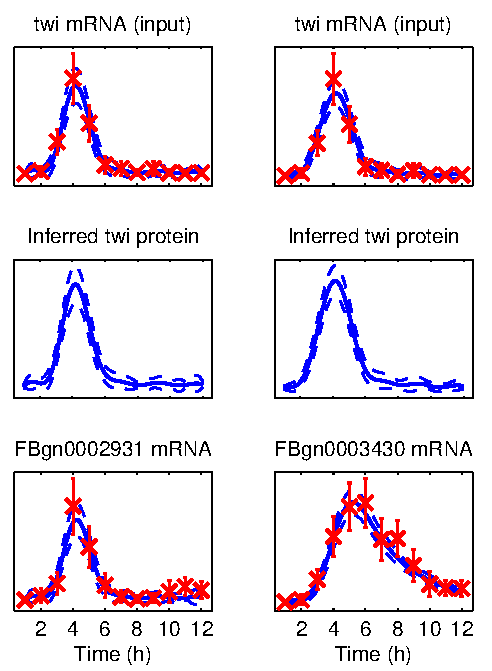
\includegraphics{gpdisim_models_twi}
  \caption{Two independent example Gaussian process models for likely
    targets of Twist. Red marks denote observed expression levels with
    2 s.d.\ error bars while blue functions are inferred from the
    model.  The dashed lines denote 2 s.d.\ confidence intervals.}
  \label{fig:gpdisim_models}
\end{figure}

We fitted two sets of Gaussian process models to Drosophila
developmental microarray time series from~\cite{Tomancak2002} using
Twist and Mef2 as TFs independently and all other genes as candidate
targets.  Quiet candidate targets with insufficient support for
regulation were eliminated as described in Materials and Methods.
Because Twist and Mef2 are known to be mainly active in mesoderm and
muscle development, the candidate genes were further pruned by only
including those with annotated expression in these tissues in the
\emph{in situ} data from~\cite{Tomancak2002} for validation.
This evaluation corresponds to
the situation in typical cell culture studies, where all active genes
are known to be localized to the same cells.
Two
examples of these models for likely Twist targets are displayed in
Fig.~\ref{fig:gpdisim_models}.

The remaining candidate targets were ranked by model likelihood.  For
comparison, candidates were also ranked by correlation of the
expression profile with the TF expression profile (``correlation'')
and by $q$-value of differential expression
from~\cite{Sandmann2006a,Sandmann2007a} (``knock-out'').

\begin{figure}[htb]
  \centering
  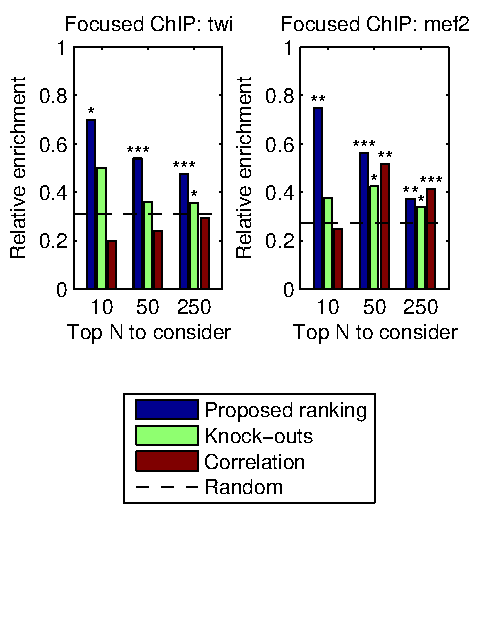
\includegraphics[trim=0mm 15mm 0mm 0mm]{dros_focused_evaluation}
  \caption{Evaluation results of different rankings as
    discussed in the text showing the relative frequency of positive
    predictions among $N$ top-ranking targets.  The dashed line
    denotes the frequency in full population.  The figure shows the
    frequency of
    targets with ChIP-chip binding within 5 kb of the gene.
    %$p$-values of significant results are denoted by '***': $p <
    %0.001$, '**': $p < 0.01$, '*': $p < 0.05$.
    The largest number of targets is smaller for Mef2 because there
    are only 200 positive examples in this subset of the data.}
  \label{fig:dros_focused_evaluation}
\end{figure}

The accuracy of the ranking was first evaluated by looking at the
fraction of $N$ top-ranking targets with ChIP-chip binding inside the
gene or within 5000 base pairs of its beginning or end in the data
from~\cite{Sandmann2006a,Sandmann2007a}.  For Mef2, this frequency is
only computed for genes in the part of the genome covered by the
ChIP-chip data.
These results are illustrated in Fig.~\ref{fig:dros_focused_evaluation}.
The results show that the proposed method clearly outperforms all the
tested alternatives.

\begin{figure}[htb]
  \centering
  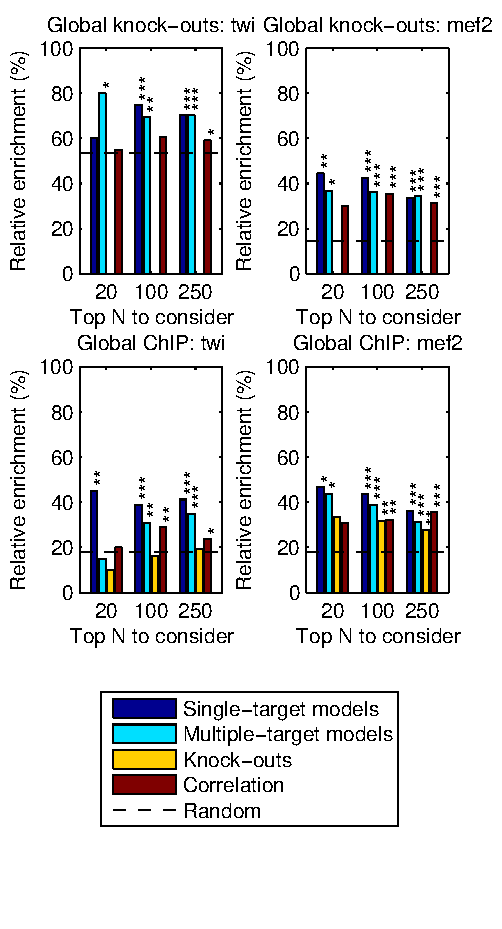
\includegraphics[trim=0mm 13mm 0mm 0mm]{dros_global_evaluation}
  \caption{Global evaluation results of different rankings as
    discussed in the text showing the relative frequency of positive
    predictions among $N$ top-ranking targets.  The dashed line
    denotes the frequency in full population.  The first row shows the
    frequency of predicted targets with in-situ annotations for
    mesoderm and muscle while the second row shows the frequency of
    targets with ChIP-chip binding within 5 kb of the gene.
    %$p$-values of significant results are denoted by '***': $p <
    %0.001$, '**': $p < 0.01$, '*': $p < 0.05$.
  }
  \label{fig:dros_global_evaluation}
\end{figure}

The accuracy of the ranking was also evaluated by looking at the
global fraction of $N$ top-ranking targets regardless of the
\emph{in situ} annotations
with annotated expression in
mesoderm and muscle tissues where the TFs are known to operate in data
from~\cite{Tomancak2002}.  These results are illustrated on the first
row of Fig.~\ref{fig:dros_global_evaluation}.  The second row of the
figure shows similar validation using the fraction of globally top-ranking
targets with ChIP-chip binding inside the gene or within 5000 base
pairs of its beginning or end in the data
from~\cite{Sandmann2006a,Sandmann2007a}.  For Mef2, this frequency is
again only computed for genes in the part of the genome covered by the data.

The results for $N=10$ are only significantly better than random for
Twist ChIP-chip, while for $N=50$ and especially $N=250$ the
improvement is highly significant.  Especially for Twist the results
are even now clearly better than any of the tested alternatives.

We also repeated the experiment with the method of~\cite{Gatta2008}
but using the TF expression levels as a proxy for the measured protein
levels.  The results of this method are significantly better than
random only for Mef2 with $N=250$ and in one evaluation with $N=50$.
Using measured protein levels would naturally help, but unfortunately
they are not available in this case.

\section{Discussion}

The linear differential equation model is a simplification, and in
many cases unrealistic. It is, however, necessary to keep the
computational load at a level that allows performing the ranking in a
workstation rather than a supercomputer.

\begin{materials}
  \section{Expression data preprocessing} Drosophila developmental
  microarray time series from~\cite{Tomancak2002} were reprocessed
  using mmgMOS from the puma package~\cite{Pearson2009}.  The means of
  the log-scale expression values were equalized across chips.  The
  distributions over log-expression were transformed to means
  ($\hat{m_i}(t_j), \hat{f_i}(t_j)$) and variances ($\sigma^m_{ij},
  \sigma^f_{ij}$) of absolute expression by minimizing the squared
  deviation of 5\%, 25\%, 50\%, 75\% and 95\% quantiles of a Gaussian
  distribution to corresponding quantiles from mmgMOS.

  \section{Covariance of the Gaussian Process}
  Differential
  equations~[\ref{eq:translation_ode}--\ref{eq:transcription_ode}]
  can be solved to obtain
  \begin{align*}
    %\label{eq:gpsim_f_ode_sol}
    p(t) &= \sigma \exp(-\delta t) \int_0^t f(v) \exp(\delta v) dv\ , \\
    m_j(t) &= \frac{B_j}{D_j} + S_j \exp(-D_j t) \int_0^t p(u)
    \exp(D_j u) du\ .
    %\label{eq:gpsim_f_x_sol}
  \end{align*}
  Using these solutions and assuming a squared exponential covariance
  for $f(t)$, $k_{ff}(t, t') = a \exp\left( -\frac{(t-t')^2}{l^2}
  \right)$, the covariance of target mRNAs is
  \begin{multline*}
    k_{m_j m_k}(t, t')
    = \frac{\sqrt{\pi} l a^2 \sigma^2 S_j S_k}{2} \bigg(
    h_{kj}(t, t', \delta) + h_{jk}(t', t, \delta) \\
    - h_{kj}(t, t', D_j) - h_{jk}(t', t, D_k)
    \bigg)\ ,
  \end{multline*}
  where
  \begin{multline*}
    h_{kj}(t, t', D_x) = 
    \exp\left(\left(\frac{D_x l}{2}\right)^2\right)
    \frac{\exp(-D_x t - D_k t')}{(D_x + \delta) (D_j - \delta)}
    \bigg\{ 
    \\
    % \frac{(D_k + \delta)\exp((D_k-\delta) t') - 2\delta}{(D_k^2-\delta^2)}
    \left(\frac{\exp((D_k-\delta) t') - 1}{D_k-\delta} +
      \frac{1}{D_k + D_x} \right)
    [\erf(\frac{D_x l}{2} - \frac{t}{l}) - \erf(\frac{D_x l}{2})]
    \\
    + \frac{\exp((D_k+D_x)t')}{D_k+D_x}
    [\erf(\frac{D_x l}{2} + \frac{t'}{l})
    - \erf(\frac{D_x l}{2} - \frac{t-t'}{l})]
    \bigg\}\ .
  \end{multline*}
  Denoting $\Delta t := t - t'$, we obtain similarly
  \begin{multline*}
    k_{f m_k}(t, t')
    = \sigma S_k a^2 \frac{\sqrt{\pi} l}{2(\delta - D_k)} \\
    \bigg(
    \exp\left(\left(\frac{D_k l}{2}\right)^2 + D_k \Delta t \right)
    [\erf(\frac{D_k l}{2} + \frac{t}{l}) - \erf(\frac{D_k l}{2} + \frac{\Delta t}{l})] \\
    -
    \exp\left(\left(\frac{\delta l}{2}\right)^2 + \delta \Delta t\right)
    [\erf(\frac{\delta l}{2} + \frac{t}{l}) - \erf(\frac{\delta l}{2} + \frac{\Delta t}{l})]
    \bigg)
  \end{multline*}

  \section{Filtering quiet genes}
  The Gaussian process model gives a high likelihood to many targets
  with very little activity that fit a constant response.  These genes
  were eliminated from the ranking by discarding targets with a higher
  likelihood for a model using only Eq.~(\ref{eq:transcription_ode})
  with $S=0$ that for the full model.
  
\end{materials}

\begin{acknowledgments}
A.H. was supported by a postdoctoral researcher's project of the Academy of Finland.
M.R. and N.D.L acknowledge support from EPSRC Grant No EP/F005687/1 "Gaussian Processes for Systems Identification with Applications in Systems Biology". 
This work was supported in part by the IST Programme of the European Community, under the PASCAL2 Network of Excellence, IST-2007-216886. This publication only reflects the authors' views.
\end{acknowledgments}

\bibliographystyle{pnas}
\bibliography{disim}

%\begin{thebibliography}{10}
%\bibliography{puma_package}
%\end{thebibliography}
\end{article}

% Figures


\end{document}


